% !TEX root = ../Projektdokumentation.tex
\section{Implementierungsphase} 
\label{sec:Implementierungsphase}

Bevor mit der Implementierung begonnen wurde, wurde ein Iterationsplan erstellt. In diesem wurden die einzelnen Schritte und deren Reihenfolge festgelegt. In jeder Iteration wurde eine spezifische Funktionalität umgesetzt und am Ende der jeweiligen Iteration dem Team präsentiert. Dieses Vorgehen folgt den in Abschnitt 2.3 beschriebenen Prinzipien der agilen Softwareentwicklung. Der vollständige Iterationsplan befindet sich im \Anhang{app:Iterationsplan}.

\subsection{Implementierung der GitLab Systemhook}
\label{sec:ImplementierungGitlabSystemhook}

Im Rahmen der Implementierung der GitLab Systemhook wurde ein Prozess entwickelt, der es ermöglicht, Ereignisse wie die Erstellung neuer Benutzer in GitLab zu erfassen und an ein SNS (Simple Notification Service) Topic weiterzuleiten. Dabei stand im Vordergrund, die Systemhook effizient, erweiterbar und in der Lage zu gestalten, Echtzeit-Benachrichtigungen für verschiedene GitLab-Ereignisse zu verarbeiten.

\begin{figure}[htb]
    \centering
    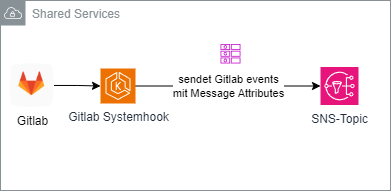
\includegraphics[scale=0.5]{systemhookOnly.drawio.png}
    \caption{Implementierung der GitLab Systemhook}
\end{figure}

Das \texttt{Hook}-Struct sowie die Initialisierung der erforderlichen Komponenten, wie dem GitLab-Client und dem AWS SNS-Client, wurden gemäß den Anforderungen definiert. Der Endpunkt, an den die HTTP-POST-Anfragen gesendet werden, ist \texttt{/api/v1/hook}. Dieser wird durch die Methode \texttt{handleHook} in der \texttt{Hook}-Struktur verarbeitet, die im Anhang~\ref{app:Test} dargestellt wird. Der Ablauf beginnt mit der Authentifizierung der HTTP-POST-Anfragen durch die Überprüfung des Tokens, um sicherzustellen, dass nur autorisierte Systeme Zugriff auf die Webhook-API erhalten. Codeauschnitte des
Authentifizierung-
sprozesses befinden sich im Anhang~\ref{app:CNMI}.

Sobald ein GitLab-Ereignis erkannt wurde, erfolgt die Verarbeitung der Payload asynchron. Durch die asynchrone Verarbeitung werden eingehende Anfragen schnell entgegengenommen und weiterverarbeitet, ohne das System zu blockieren. Im nächsten Schritt wird die empfangene Payload an den SNS-Dienst gesendet, wie in Anhang~\ref{app:CNMI} veranschaulicht. Damit die Nachrichten gezielt gefiltert und ausgewertet werden können, werden sogenannte \texttt{MessageAttributes} erstellt. Diese Attribute enthalten Informationen über das jeweilige Ereignis, wie z.B. den Ereignisnamen oder spezifische Merkmale des Benutzers, der das Ereignis ausgelöst hat. Im Falle einer Benutzererstellung wird beispielsweise geprüft, ob der neue Benutzer ein Bot ist, was ebenfalls als Attribut weitergeleitet wird.

Die \texttt{MessageAttributes} spielen eine entscheidende Rolle bei der Filterung und ermöglichen eine granulare Weiterleitung von GitLab-Ereignissen. Auf Basis dieser Attribute können spezifische Filter Policies angewendet werden, sodass nur relevante Events an nachgelagerte Systeme oder Prozesse weitergeleitet werden.



\subsection{Implementierung des Dev-Kickstarter}
\label{sec:ImplementierungBenutzeroberflaeche}

Im Rahmen der Implementierung des Dev-Kickstarter wurde eine robuste Architektur entworfen, die es ermöglicht, verschiedene Benutzerereignisse zu verarbeiten und Aktionen wie das Versenden von Willkommens-E-Mails und das Hinzufügen neuer Benutzer zu Microsoft Teams-Gruppen automatisiert auszuführen.

\begin{figure}[htb]
    \centering
    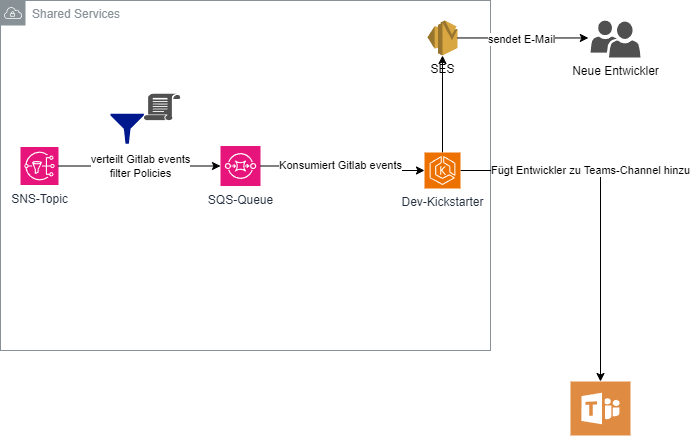
\includegraphics[scale=0.5]{dev-kickstarterOnly.drawio.png}
    \caption{Implementierung des Dev-Kickstarter}
\end{figure}

Das \texttt{Kickstarter}-Struct sowie die Initialisierung der erforderlichen Komponenten, wie dem AWS SES-Client, SQS-Consumer und Microsoft Graph-Client, wurden gemäß den Anforderungen definiert. Der SQS-Consumer empfängt Nachrichten aus einer AWS SQS-Queue, die mit Filter Policies erstellt wurde, um nur relevante Ereignisse zu verarbeiten. Die Definition der \texttt{Kickstarter}-Struktur ist im Anhang~\ref{app:kickStruct} zu finden.

Nach dem Empfang einer Nachricht wird die Payload asynchron verarbeitet. Dabei wird die E-Mail-Adresse des Benutzers extrahiert, um eine Willkommens-E-Mail über den AWS SES-Dienst zu versenden. Der zugehörige Code befindet sich im Anhang~\ref{app:kickMain}. Anschließend wird der Benutzer automatisch zu einer definierten Microsoft Teams-Gruppe hinzugefügt, indem die Microsoft Graph API verwendet wird.


\subsection{Implementierung der E-Mail}
\label{sec:ImplementierungGeschaeftslogik}

Die E-Mail wurde als HTML-Dokument erstellt, um sicherzustellen, dass sie auf verschiedenen Endgeräten und E-Mail-Clients korrekt angezeigt wird. Dabei wurde inline CSS verwendet, da viele E-Mail-Clients externe Stylesheets nicht vollständig unterstützen. Dies gewährleistet eine konsistente Darstellung der E-Mail auf allen Plattformen.

Ein wichtiges Merkmal der Implementierung ist die dynamische Personalisierung der Inhalte. Dazu wurde der Platzhalter \texttt{\{\{.FirstName\}\}} eingefügt, um den Vornamen des Empfängers einzufügen. Dieser Wert wird zur Laufzeit gefüllt, indem der Code des Empfängers ausgewertet und der entsprechende Vorname dynamisch in die Vorlage eingefügt wird.

Zusätzlich wurden nützliche Ressourcen und Links in die E-Mail integriert, wie z.B. der Zugriff auf interne TUI-Plattformen wie \textit{Runway} und \textit{OneSource}, um den neuen Teammitgliedern den Einstieg zu erleichtern. Sicherheitsaspekte wurden ebenfalls berücksichtigt, indem Links zu den TUI-Sicherheitsrichtlinien eingebunden wurden. Dies unterstreicht die Wichtigkeit des sicheren Arbeitens innerhalb der Organisation.

Wie die finale E-Mail aussieht, kann im Anhang~A.\ref{app:finalDesign} eingesehen werden.



